\chapter{Methodology}
\section{The data and tools}
    The data was provided by the \gls{imr} and I had access to a broad selection of yearly trawl cruises spanning from 2011 to 2020. In this chapter, I will delve into the data itself to give you a clearer picture of how I looks, how I acquired it and what tools I utilized.
    
    \subsection{The data provided (.RAW)}
        The files were initially presented to me as ".RAW" \cite{raw} and ".WORK" files. ".RAW" is the uncompressed raw output from the echo sounder. The same format is used by cameras before they are converted to, for example, ".JPEG". Because they are uncompressed, they do not lose any data. Unfortunately, this also makes them large. The ".WORK" files are the annotations of the ".RAW" files done by operators using a system called the \Gls{lsss}\cite{lsss}. The data from 2020 alone which spanned three months took 240 GB of storage space and stored on a remote server.
        
        SJEKK DATAEKSEMPEL!
    \subsection{Windows Azure}
        Windows Azure \cite{azure} is a platform owned by Microsoft that provides cloud solutions for several services. My use was to access a remote storage provided by the \gls{imr} and mount this to my local computer. Thus enabling me to download the data for this thesis from \gls{imr}s server. 
    
    \subsection{Docker}
        Docker \cite{docker} is an open source platform that provides what they call containerization and is owned by the company under the same name, Docker, Inc. If you are familiar with virtual machines, then containerization will be very familiar to you. Docker is based on the Linux kernel, and enables you to create a container, which is an independent process that uses resources from the main instance. For each container, you can manage its own dependencies like programming languages and libraries. These containers can then be shared with others as images files, and as they can be run without the receiver having to manage the aforementioned dependencies as this is built into the image. Thus, you can make an application or code easily accessible for other people, as long as they have installed Docker.
        
    \subsection{Zarr}
        By using the ".ZARR" \cite{zarr} format, you gain access to store chunked compressed  multidimensional arrays. There are several highlights from this library, but I used primarily the ability to access the arrays on disk. This means I did not need to load the entire array into memory and could work with the array and access parts of it without hardware limitations.
        
    \subsection{CRIMAC-pipeline} \label{CRIMAC-pipeline}
        Together, the \gls{nr} and the \gls{imr} developed a pipeline\cite{crimac_pipeline} to classify the acoustic backscatter in echo sounder data. This was part of the work described earlier in \ref{unet_paper_acoustic} and is accessed by using docker. They also provide the image for a container to access the data through Azure.
        
        The pipeline is run using one docker container, which in turn downloads and runs four others:
        
            \begin{description}
              \item[$\bullet$ Preprocessor] Preprocesses the ".RAW" and ".WORK" to respectively ".ZARR" and ".PARQUET" files. Since frequencies can have different resolutions, all are re-gridded to the 38kHz frequency.
              \item[$\bullet$ Unet] Using a pretrained deep learning model called Unet it produces pixel based annotations
              \item[$\bullet$ Bottom detection] Identifies the bottom and generates a pixel based map stored as ".ZARR".
              \item[$\bullet$ Report generation] Takes in the output from the bottom detection, Unet and the preprocessed ".RAW" file and generates a report for the \gls{ices}.
    
            \end{description}
        
        The Unet, bottom detection and preprocessing is the same as described in section \ref{unet_paper_acoustic}.

    \subsection{Xarray}
        Xarray\cite{xarray} is a Python package that is made for working with multidimensional arrays. It is based on NumPy and adds labels in the form of attributes and coordinates on top of the NumPy-arrays. This was the library I used for accessing and working more efficiently with the ".ZARR" arrays, as I was already very familiar with NumPy.


        
\section{Challenges}
    \subsection{The ZARR issue}
        things
    \subsection{Bitmap errors} \label{bitmap_error}
        things

\section{My solution}
    \subsection{Pseudo labels}\label{Pseudo label}
        Due to the bitmap errors mentioned in \ref{bitmap_error} I did not have access to the same labels that were used in the original work \ref{unet_paper_acoustic} and so had to find an alternate solution. This came to be based on what is called pseudo labels. In meetings with the \gls{imr} we came up with the idea to use the output of the model used in \ref{unet_paper_acoustic} as my labels. This was based on the fact that the models' performance were assessed to be sufficient for my task. I was then able to create as much data with corresponding pseudo labels as I deemed necessary.
        
    \subsection{The final dataset}
        With the pseudo labels from section \ref{Pseudo label} I possessed all the components I needed to create my own dataset. Here I will go through my implementation of preprocessing the ".RAW" into a dataset able to be quickly loaded into a deep learning algorithm.
        
        \begin{figure}[H]
            \centering
            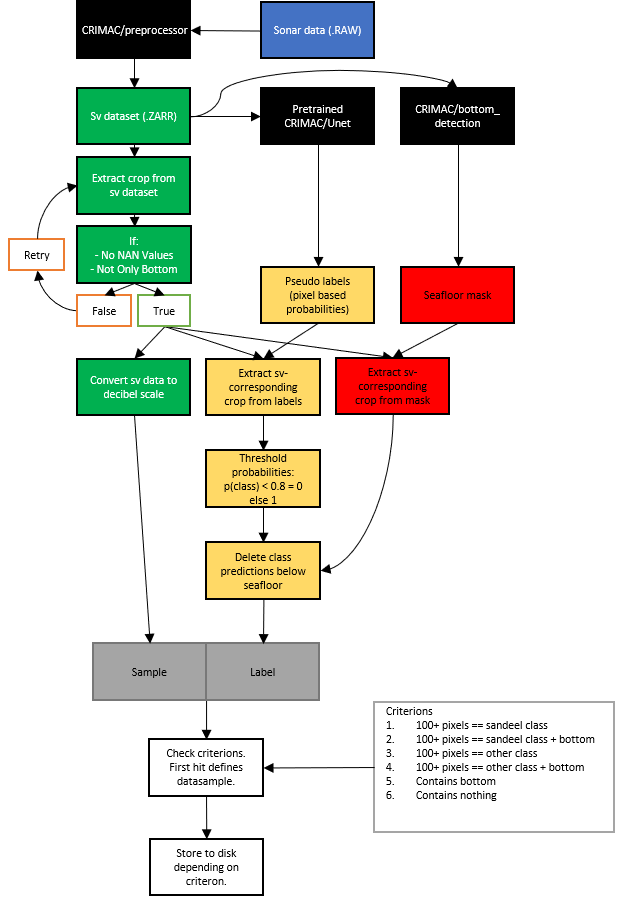
\includegraphics[scale=0.8]{figures/flow_data_gen.png}
            \caption{An overview of the data generation process. CRIMAC pipeline module (black), data.raw (blue), data.zarr (green), pseudo labels (yellow), bottom (red) and the finished file (gray)}
          	\medskip 
            \label{data_generation_flowchart_fig}
        \end{figure}
        
        The entire process is illustrated in figure \ref{data_generation_flowchart_fig} and starts with the utilization of \gls{crimac} preprocessor module as described in \ref{CRIMAC-pipeline}. This takes in the .RAW data and outputs the sv data in the .zarr format. Following the \gls{sv} data, a crop is then extracted was checked for missing values and if it contained only data from below the seafloor. This is repeated until it find one that is valid. 
        
        In figure \ref{data_generation_flowchart_fig} the  \gls{sv} data were also sent to both the pretrained Unet and bottom detection modules from the \gls{crimac} pipeline. The Unet outputs the pseudo labels and the bottom detection outputs a mask of the seafloor. Then the same crop that were extracted from the \gls{sv} data were extracted from both the seafloor mask and 
        
        
        
        
        
        The final product was individual files containing a single data sample with all frequencies that were previously in the ".raw" file and a corresponding pseudo label. The file was then stored using pytorch based on some criterions that will be explained shortly, creating a data hierarchy as shown in figure \ref{data_hierarchy_fig}:
        
        \begin{figure}[H]
            \centering
            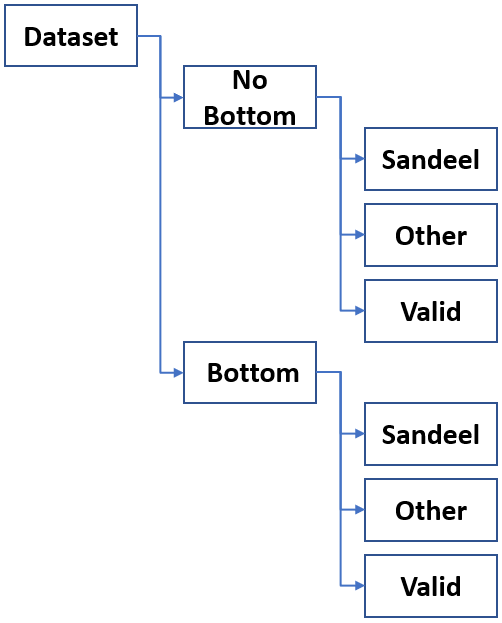
\includegraphics[scale=0.5]{figures/data_hierarki.png}
            \caption{An overview of the data hierarchy.}.
          	\medskip 
            \label{data_hierarchy_fig}
        \end{figure}
        
        The criterions were based on those stated in the \ref{unet_paper_acoustic} article and can be seen in figure \ref{data_generation_flowchart_fig}. In the previously mentioned article, they had the real labels to know if there was "sandeel" or instances of the "other" class in a crop. I had to rely on the pseudo labels for the same task, and this introduced noise. Hence, I set a filter where 100 of the pixels in the crop had to belong to a single class to satisfy my criteria. 
        
        
        
        
        
        HERE COME MORE OF THE CHECKS FOR BOTTOM, SANDEEL and stuff.
        


\section{Experiments}
    \subsection{Greedy-search frequencies}
        things
    